\section{EXPERIMENT} \label{sec:exp}

We evaluate \solution on two widely-acknowledged public benchmarks: DWY100K and DBP15K. DWY100K is a monolingual dataset and DBP15K is a multi-lingual dataset.   

%\subsection{Experiment Setup}

\vpara{DWY100K.} The DWY100K dataset used here is originally built by~\cite{sun2018bootstrapping}. DWY100K consists of two large datasets: DWY100K$_{\text{dbp\_wd}}$ (DBpedia to Wikidata) and DWY100K$_{\text{dbp\_yg}}$ (DBpedia to YAGO3). Each dataset contains 100,000 pairs of aligned entities. However, the entity in the "wd" (Wikidata) part of DWY100K$_{\text{dbp\_wd}}$ are represented by indices (e.g., Q123) instead of URLs containing entity names, and we search their entity names via the Wikidata\footnote{\url{https://pypi.org/project/Wikidata/}} API for python.
%To leverage the entity names, we need to use the current Wikidata to map the indices to string names. As a result, we find ten entity indices in the "wd" (Wikidata) as a part of DWY100K$_{\text{dbp\_wd}}$ are no longer presented in Wikidata now. We delete those entities and replace others with corresponding 

\begin{table}[t]
\centering
\renewcommand\tabcolsep{9pt}
  \caption{
    Statistics of DWY100K and DBP15K. \textmd{About the definition of neighbor similarity, please refer to Section~\ref{sec:exp}. ``\#Link" is the number of aligned entity pairs. ``\#Test Link" is the number of aligned pairs for test.}
    }
    \label{data}
    \scalebox{0.8}{
  \begin{tabular}{@{}cccccc@{}}
      \toprule[1.5pt]
      \multirow{2}{*}{Model} & \multicolumn{2}{|c|}{DWY100K}  & \multicolumn{3}{c}{DBP15K} \\ \cmidrule(l){2-6} 
                         %\\ \midrule
                         & \multicolumn{1}{|c}{dbp\_wd} & \multicolumn{1}{c}{dbp\_yg} & 
                         \multicolumn{1}{|c}{zh\_en} & 
                         \multicolumn{1}{c}{ja\_en} & 
                         \multicolumn{1}{c}{fr\_en} \\ 
    \midrule
        \multicolumn{1}{c|}{\#Link} &
        \multicolumn{1}{c}{99990} &
        \multicolumn{1}{c|}{100000} & 
        \multicolumn{1}{c}{15000} &
        \multicolumn{1}{c}{15000} &
        \multicolumn{1}{c}{15000} \\ 
    \midrule
        \multicolumn{1}{c|}{\#Test Link} &
        \multicolumn{1}{c}{69993} &
        \multicolumn{1}{c}{70000} &
        \multicolumn{1}{|c}{10500} &
        \multicolumn{1}{c}{10500} &
        \multicolumn{1}{c}{10500} \\
    \midrule
        \multicolumn{1}{c|}{\shortstack{neighbor similarity}} &
          \multicolumn{1}{c}{0.633} &
          \multicolumn{1}{c|}{0.777} &
          \multicolumn{1}{c}{0.418} &
          \multicolumn{1}{c}{0.188} &
          \multicolumn{1}{c}{0.182} \\
      \bottomrule[1.5pt]
     \end{tabular}
     }
    \label{tab:stats}
    \vspace{-0.3cm}
\end{table}

\vpara{DBP15K.} The DBP15K dataset is originally built by~\cite{JAPE}\footnote{\url{https://github.com/nju-websoft/JAPE}} and translated into English by~\cite{xu2019cross-lingual}. The DBP15K consists of three cross-lingual datasets: DBP15K$_{\text{zh\_en}}$ (Chinese to English), DBP15K$_{\text{ja\_en}}$ (Japanese to English) and DBP15K$_{\text{fr\_en}}$ (French to English). All three datasets are created from multi-lingual DBpedia, and each contains 15,000 pairs of aligned entities. 
%As~\cite{JAPE} explained in their GitHub repository\footnote{\url{https://github.com/nju-websoft/JAPE}}, they do not use all the triples in the original DBP15K dataset they built: for relationship triples, they select a portion whose head and tail entities are popular. A translated-to-English version is provided by~\cite{xu2019cross} and used by several baselines. 
We report results on both original and translated version.

%\vpara{FW1M.} To examine \solution and baselines' abilities to scale up, we present a new web-scale multi-lingual entity alignment dataset---FW1M---which contains 5.6 million entities, 22.8 million triples from Freebase and 2.4 million entities, 13.2 million triples from Wikidata. In 2015, Freebase is migrated to Wikidata by Google~\cite{pellissier2016freebase}, during which high quality aligned pairs were produced by original hyperlinks and crowd-sourcing. In Wikidata, the property ``Freebase ID'' records this aligned relationships, and we extract 1.25 million aligned pairs as the groundtruth. To make FW1M a multi-lingual one, considering the poorest performed dataset in DBP15K is DBP15K$_{\text{zh\_en}}$, for those entities with both English and Chinese aliases, we randomly select one of them as the entity name.

The statistics of DWY100K and DBP15K we use in our work are shown in Table \ref{tab:stats}. 
Beyond basic information, we also present a study on datasets' average (1-hop) neighbor similarity, which is the ratio of aligned neighbors of a pair of aligned entities, indicating how noisy the neighborhood information is.
We observe that DWY100K's neighborhood information is quite useful, while DBP15K's neighborhood information can be very noisy.

\vpara{Experiment Setup.}
We follow the original split of DWY100K \cite{sun2018bootstrapping} and DBP15K \cite{JAPE} which are shown in Table \ref{tab:stats}. 
For \solution, we randomly take out 5\% from the original training set as a dev set for early stopping. 
We use Hit@$k$ $(k=1, 10)$ to evaluate our model's performance as most works do. 
The similarity score is calculated using the $\ell_2$ distance of two entity embeddings. The batch size is set to 64, momentum $m$ is set to $0.9999$, temperature $\tau$ is set to $0.08$, and queue size is set to 64. We use a learning rate of $10^{-6}$ with Adam on a Ubuntu server with NVIDIA V100 GPUs (32G).

%From the values of "Levenshtein distance Hit@k" in Table \ref{data}, it is surprising to see that character-level similarity is such a strong baseline. With the Hit@1 of 0.863 and 1.000, the result based on such a traditional approach outperforms many recent supervised entity alignment approaches by a large margin, including RDGCN~\cite{wu2019relation} and NAEA~\cite{zhu2019neighborhood}. However, it is time-consuming to calculate pairwise Levenshtein distance, and modern embedding-based methods can perform fast ranking using vector searching tools such as the Faiss\footnote{https://github.com/facebookresearch/faiss}. However, it still reminds us of the importance of including character-level information in the monolingual entity alignment.

%For baselines, because of the limited passage length, we will introduce them in the Appendix \ref{app:baseline}.
%\zfj{you haven't introduce baseline methods in the big tables.}





\subsection{Results}

In this part, we report the results of \solution and baselines on DWY100K and DBP15K. For all the baselines, we take the reported scores from the corresponding papers, or directly from the tables in BERT-INT~\cite{tang2019bert-int}, CEAFF~\cite{CEAFF} or NAEA~\cite{zhu2019neighborhood}. According to the used proportion of the training labels, we categorize all the models into two types:
\begin{itemize}
    \item Supervised: 100\% of the aligned entity links in the training set is leveraged
    \item Unsupervised \& Self-supervised: 0\% of the training set is leveraged.
\end{itemize}


%Another surprising finding is that , when training \solutionchar on DWY100K$_{\text{dbp\_yg}}$, the Hit@1 and Hit@10 will reach 1.000 after only one epoch of training, indicating that \solutionchar is very powerful at extracting character-level information.

%We also notice the difference between \solutionchar and \solutionsem, that \solutionchar performs a little bit poorer by 2\%. However, this is understandable because \solutionsem is not only capable of grasping semantic-level information essential for entity alignment, but also it can capture the character-level information to some extent. This is because the tokenizer for BERT-style language models is implemented by WordPiece~\cite{wu2016google} algorithm, which would split uncommon words into segments of characters. The WordPiece algorithm is based on byte pair encoding, which split a sentence by white spaces and also an integral word into subwords. For example, an entity named ``Novak Djokovic'' would be split into \{`Novak', `D', `\#\#jo', `\#\#kovic'\}, which also well preserves the character-level information.

%However, \solutionchar has its unique advantage, that it has a much smaller model size, higher training speed and higher inference speed, which would be super important when it comes to the large-scale dataset. LaBSE is a fine-tuned version of multi-lingual BERT with 110M parameters. Meanwhile, the \solutionchar only employs about 0.1M parameters, which is several magnitudes smaller than \solutionsem.

\begin{table}[t]
	\centering
	\renewcommand\tabcolsep{9pt}
	\renewcommand\arraystretch{0.95}
	\caption{Results on DWY100K. \textmd{Bold results are our best result; underline results are best baseline results.}}
	\scalebox{0.8}{
      \begin{tabular}{@{}cccccc@{}}
          \toprule[1.2pt]
          \multirow{2}{*}{Model} &
            \multicolumn{2}{|c|}{DWY100K$_{\text{dbp\_wd}}$} &
            \multicolumn{2}{|c|}{DWY100K$_{\text{dbp\_yg}}$} &
            \multirow{2}{*}{\makecell[c]{macro\\Hit@1}} \\ 
            \cmidrule(l){2-5} 
           &
            \multicolumn{1}{|c}{Hit@1} &
            \multicolumn{1}{c|}{Hit@10} &
            \multicolumn{1}{c}{Hit@1} &
            \multicolumn{1}{c|}{Hit@10} \\ 
            \midrule
          \multicolumn{6}{c}{Supervised}                     \\ 
          \midrule
          \multicolumn{1}{c|}{MTransE~\cite{MTransE}} &
            \multicolumn{1}{c}{0.281} &
            \multicolumn{1}{c|}{0.520} &
            \multicolumn{1}{c}{0.252} &
            \multicolumn{1}{c|}{0.493} &
            \multicolumn{1}{c}{0.267} \\ \midrule
            \multicolumn{1}{c|}{JAPE~\cite{JAPE}} &
            \multicolumn{1}{c}{0.318} &
            \multicolumn{1}{c|}{0.589} &
            \multicolumn{1}{c}{0.236} &
            \multicolumn{1}{c|}{0.484} &
            \multicolumn{1}{c}{0.277} \\ \midrule
            \multicolumn{1}{c|}{IPTransE~\cite{zhu2017iterative}} &
            \multicolumn{1}{c}{0.349} &
            \multicolumn{1}{c|}{0.638} &
            \multicolumn{1}{c}{0.297} &
            \multicolumn{1}{c|}{0.558} &
            \multicolumn{1}{c}{0.322} \\ \midrule
            \multicolumn{1}{c|}{GCN-Align~\cite{GCN-Align}} &
            \multicolumn{1}{c}{0.477} &
            \multicolumn{1}{c|}{-} &
            \multicolumn{1}{c}{0.601} &
            \multicolumn{1}{c|}{-} &
            \multicolumn{1}{c}{0.539}\\ \midrule
            \multicolumn{1}{c|}{MuGNN~\cite{cao2019multi}} &
            \multicolumn{1}{c}{0.616} &
            \multicolumn{1}{c|}{0.897} &
            \multicolumn{1}{c}{0.741} &
            \multicolumn{1}{c|}{0.937} &
            \multicolumn{1}{c}{0.679}\\ \midrule
            \multicolumn{1}{c|}{RSNs~\cite{guo2019learning}} &
            \multicolumn{1}{c}{0.656} &
            \multicolumn{1}{c|}{-} &
            \multicolumn{1}{c}{0.711} &
            \multicolumn{1}{c|}{-} &
            \multicolumn{1}{c}{0.684}\\ \midrule
            \multicolumn{1}{c|}{BootEA~\cite{sun2018bootstrapping}} &
            \multicolumn{1}{c}{{0.748}} &
            \multicolumn{1}{c|}{0.898} &
            \multicolumn{1}{c}{{0.761}} &
            \multicolumn{1}{c|}{0.894} &
            \multicolumn{1}{c}{0.755}\\ \midrule
            \multicolumn{1}{c|}{NAEA~\cite{zhu2019neighborhood}} &
            \multicolumn{1}{c}{0.767} &
            \multicolumn{1}{c|}{0.918} &
            \multicolumn{1}{c}{0.779} &
            \multicolumn{1}{c|}{0.913} &
            \multicolumn{1}{c}{0.773}\\ \midrule
            
            \multicolumn{1}{c|}{TransEdge~\cite{sun2019transedge}} &
            \multicolumn{1}{c}{0.788} &
            \multicolumn{1}{c|}{0.938} &
            \multicolumn{1}{c}{0.792} &
            \multicolumn{1}{c|}{0.936} &
            \multicolumn{1}{c}{0.790}\\ \midrule
            
            \multicolumn{1}{c|}{RDGCN~\cite{wu2019relation}} &
            \multicolumn{1}{c}{0.902} &
            \multicolumn{1}{c|}{-} &
            \multicolumn{1}{c}{0.864} &
            \multicolumn{1}{c|}{-} &
            \multicolumn{1}{c}{0.883}\\ \midrule
            \multicolumn{1}{c|}{COTSAE~\cite{yang2020cotsae}} &
            \multicolumn{1}{c}{0.927} &
            \multicolumn{1}{c|}{0.979} &
            \multicolumn{1}{c}{0.944} &
            \multicolumn{1}{c|}{0.987} &
            \multicolumn{1}{c}{0.936}\\ \midrule
            \multicolumn{1}{c|}{BERT-INT~\cite{tang2019bert-int}} &
            \multicolumn{1}{c}{0.992} &
            \multicolumn{1}{c|}{-} &
            \multicolumn{1}{c}{0.999} &
            \multicolumn{1}{c|}{-} &
            \multicolumn{1}{c}{0.996}\\ \midrule
            \multicolumn{1}{c|}{CEAFF~\cite{CEAFF}} &
            \multicolumn{1}{c}{\underline{1.000}} &
            \multicolumn{1}{c|}{-} &
            \multicolumn{1}{c}{\underline{1.000}} &
            \multicolumn{1}{c|}{-} &
            \multicolumn{1}{c}{1.000}\\ 
          %\midrule
          %\multicolumn{5}{c}{Semi-supervised (30\% training)}              \\ 
          \midrule
            \multicolumn{6}{c}{Unsupervised \& Self-supervised}              \\ 
            \midrule
            \multicolumn{1}{c|}{MultiKE~\cite{zhang2019multi}} &
            \multicolumn{1}{c}{0.915} &
            \multicolumn{1}{c|}{-} &
            \multicolumn{1}{c}{0.880} &
            \multicolumn{1}{c|}{-} &
            \multicolumn{1}{c}{0.898}\\ \midrule[1.3pt]
          \multicolumn{1}{c|}{\textbf{\solution}} &
            \multicolumn{1}{c}{\textbf{0.983}} &
            \multicolumn{1}{c|}{\textbf{0.998}} &
            \multicolumn{1}{c}{\textbf{1.000}} &
            \multicolumn{1}{c|}{\textbf{1.000}} &
            \multicolumn{1}{c}{0.992}\\ 
          \bottomrule[1.2pt]
         \vspace{-0.8cm}
      \end{tabular}}
	\label{tab:dwy100k}
\end{table}

\vpara{Overall performance on DWY100K.} 
%Table \ref{dwy} presents the overall entity linking performance on DWY100K, including \solution and other baselines. Since DWY100K is a monolingual dataset, both the character-level model \solutionchar and the semantic level model \solutionsem are applicable. 
From Table~\ref{tab:dwy100k}, we observe that \solution outperforms all the supervised and unsupervised models except for supervised CEAFF~\cite{CEAFF} and BERT-INT~\cite{tang2019bert-int}. However, without any supervision, \solution only falls behind supervised state-of-the-art CEAFF on DWY100K$_{\text{dbp\_wd}}$ by a minimal margin of 1.2\%. \hhy{The reason why DWY100K$_{\text{dbp\_yg}}$ enables SelfKG to achieve such high accuracy is that the names of its aligned entity pairs are of great similarity respectively, which makes this dataset more easier.} The inspiring result implies that at least for monolingual datasets like DWY100K, supervision is not quite necessary for entity alignment.



\vpara{Overall performance on DBP15K.} 
%In Table \ref{dbp}, we present the overall entity alignment performance on DBP15K. Because DBP15K is a multi-lingual dataset, the \solutionchar is not applicable since it requires both KGs to share the same character set. We only evaluate semantic level model \solutionsem on DBP15K.
For the DBP15K dataset, we find that different baselines use different versions of DBP15K in implementation. For example, BERT-INT~\cite{tang2019bert-int} uses the original multi-lingual version built by \cite{JAPE}, while some other methods including RDGCN~\cite{wu2019relation} and DGMC~\cite{fey2020deep} uses machine translation (Google translation) to translate non-English datasets (i.e., zh, ja, fr) of DBP15K into English. If DBP15K is translated, it should not be considered as a multi-lingual setting to some extend. For fair comparison, we report \solution's results on both settings.

%\newpage

\begin{table}[t]
	\centering
    \renewcommand\tabcolsep{3.5pt}
    %\setlength{\belowcaptionskip}{-0.5cm}
	\caption{Results on DBP15K. \textmd{Methods marked with ``$^*$'' use a translated version of DBP15K~\cite{xu2019cross-lingual}.Bold results are our best result; underline results are best baseline results.}}
	\renewcommand\arraystretch{0.9}
	\scalebox{0.8}{
      \begin{tabular}{@{}cccccccc@{}}
          \toprule[1.2pt]
          \multirow{2}{*}{Model} &
            \multicolumn{2}{|c|}{DBP15K$_{\text{zh\_en}}$} &
            \multicolumn{2}{|c}{DBP15K$_{\text{ja\_en}}$} &
            \multicolumn{2}{|c|}{DBP15K$_{\text{fr\_en}}$} &
            \multirow{2}{*}{\makecell[c]{macro\\Hit@1}} \\ 
            \cmidrule(l){2-7} 
           &
            \multicolumn{1}{|c}{Hit@1} &
            \multicolumn{1}{c|}{Hit@10} &
            \multicolumn{1}{c}{Hit@1} &
            \multicolumn{1}{c|}{Hit@10} &
            \multicolumn{1}{c}{Hit@1} &
            \multicolumn{1}{c|}{Hit@10} &\\ 
            \midrule
          \multicolumn{8}{c}{Supervised}                     \\ 
          \midrule
          \multicolumn{1}{c|}{\begin{tabular}[c]{@{}c@{}}MTransE~\cite{MTransE} \end{tabular}} &
            \multicolumn{1}{c}{0.308} &
            \multicolumn{1}{c|}{0.614} &
            \multicolumn{1}{c}{0.279} &
            \multicolumn{1}{c|}{0.575} &
            \multicolumn{1}{c}{0.244} &
            \multicolumn{1}{c|}{0.556} &
            0.277\\ 
            \midrule
          \multicolumn{1}{c|}{JAPE~\cite{JAPE}} &
            \multicolumn{1}{c}{0.412} &
            \multicolumn{1}{c|}{0.745} &
            \multicolumn{1}{c}{0.363} &
            \multicolumn{1}{c|}{0.685} &
            \multicolumn{1}{c}{0.324} &
            \multicolumn{1}{c|}{0.667} &
            0.366\\
          \midrule
          \multicolumn{1}{c|}{IPTransE~\cite{zhu2017iterative}} &
            \multicolumn{1}{c}{0.406} &
            \multicolumn{1}{c|}{0.735} &
            \multicolumn{1}{c}{0.367} &
            \multicolumn{1}{c|}{0.693} &
            \multicolumn{1}{c}{0.333} &
            \multicolumn{1}{c|}{0.685} &
            0.369\\ 
          \midrule
            \multicolumn{1}{c|}{GCN-Align~\cite{GCN-Align}} &
            \multicolumn{1}{c}{0.413} &
            \multicolumn{1}{c|}{0.744} &
            \multicolumn{1}{c}{0.399} &
            \multicolumn{1}{c|}{0.745} &
            \multicolumn{1}{c}{0.373} &
            \multicolumn{1}{c|}{0.745} &
            0.395\\
            \midrule
          \multicolumn{1}{c|}{SEA~\cite{pei2019semi}} &
            \multicolumn{1}{c}{0.424} &
            \multicolumn{1}{c|}{0.796} &
            \multicolumn{1}{c}{0.385} &
            \multicolumn{1}{c|}{0.783} &
            \multicolumn{1}{c}{0.400} &
            \multicolumn{1}{c|}{0.797} &
            0.403\\
            \midrule
          \multicolumn{1}{c|}{KECG~\cite{li2019semi}} &
            \multicolumn{1}{c}{0.478} &
            \multicolumn{1}{c|}{0.835} &
            \multicolumn{1}{c}{0.490} &
            \multicolumn{1}{c|}{0.844} &
            \multicolumn{1}{c}{0.486} &
            \multicolumn{1}{c|}{0.851} &
            0.485\\ 
            \midrule
          \multicolumn{1}{c|}{MuGNN~\cite{cao2019multi}} &
            \multicolumn{1}{c}{0.494} &
            \multicolumn{1}{c|}{0.844} &
            \multicolumn{1}{c}{0.501} &
            \multicolumn{1}{c|}{0.857} &
            \multicolumn{1}{c}{0.495} &
            \multicolumn{1}{c|}{0.870} &
            0.497\\ 
            \midrule
          \multicolumn{1}{c|}{RSNs~\cite{guo2019learning}} &
            \multicolumn{1}{c}{0.508} &
            \multicolumn{1}{c|}{0.745} &
            \multicolumn{1}{c}{0.507} &
            \multicolumn{1}{c|}{0.737} &
            \multicolumn{1}{c}{0.516} &
            \multicolumn{1}{c|}{0.768} &
            0.510\\ 
            \midrule
          \multicolumn{1}{c|}{AliNet~\cite{DBLP:journals/corr/abs-1911-08936}} &
            \multicolumn{1}{c}{0.539} &
            \multicolumn{1}{c|}{0.826} &
            \multicolumn{1}{c}{0.549} &
            \multicolumn{1}{c|}{0.831} &
            \multicolumn{1}{c}{0.552} &
            \multicolumn{1}{c|}{0.852} &
            0.547\\ 
            \midrule
          \multicolumn{1}{c|}{BootEA~\cite{sun2018bootstrapping}} &
            \multicolumn{1}{c}{0.629} &
            \multicolumn{1}{c|}{0.848} &
            \multicolumn{1}{c}{0.622} &
            \multicolumn{1}{c|}{0.854} &
            \multicolumn{1}{c}{0.653} &
            \multicolumn{1}{c|}{0.874} &
            0.635\\ 
            \midrule
          \multicolumn{1}{c|}{NAEA~\cite{zhu2019neighborhood}} &
            \multicolumn{1}{c}{0.650} &
            \multicolumn{1}{c|}{0.867} &
            \multicolumn{1}{c}{0.641} &
            \multicolumn{1}{c|}{0.873} &
            \multicolumn{1}{c}{0.673} &
            \multicolumn{1}{c|}{0.894} &
            0.655\\ 
            \midrule
          \multicolumn{1}{c|}{MRPEA~\cite{shi2019modeling}} &
            \multicolumn{1}{c}{0.681} &
            \multicolumn{1}{c|}{0.867} &
            \multicolumn{1}{c}{0.655} &
            \multicolumn{1}{c|}{0.859} &
            \multicolumn{1}{c}{0.677} &
            \multicolumn{1}{c|}{0.890} &
            0.671\\ 
            \midrule
          \multicolumn{1}{c|}{JarKA~\cite{chen2020jarka}} &
            \multicolumn{1}{c}{0.706} &
            \multicolumn{1}{c|}{0.878} &
            \multicolumn{1}{c}{0.646} &
            \multicolumn{1}{c|}{0.855} &
            \multicolumn{1}{c}{0.704} &
            \multicolumn{1}{c|}{0.888} &
            0.685\\ 
            \midrule
          \multicolumn{1}{c|}{TransEdge~\cite{sun2019transedge}} &
            \multicolumn{1}{c}{{0.735}} &
            \multicolumn{1}{c|}{{0.919}} &
            \multicolumn{1}{c}{{0.719}} &
            \multicolumn{1}{c|}{{0.932}} &
            \multicolumn{1}{c}{{0.710}} &
            \multicolumn{1}{c|}{{0.941}} &
            0.721\\ 
            \midrule
          \multicolumn{1}{c|}{GM-Align~\cite{xu2019cross-lingual}} &
            \multicolumn{1}{c}{0.679} &
            \multicolumn{1}{c|}{0.785} &
            \multicolumn{1}{c}{0.740} &
            \multicolumn{1}{c|}{0.872} &
            \multicolumn{1}{c}{0.894} &
            \multicolumn{1}{c|}{0.952} &
            0.771\\
            \midrule
          \multicolumn{1}{c|}{{JAPE~\cite{JAPE} $^*$}} &
            \multicolumn{1}{c}{0.731} &
            \multicolumn{1}{c|}{0.904} &
            \multicolumn{1}{c}{{0.828}} &
            \multicolumn{1}{c|}{0.947} &
            \multicolumn{1}{c}{-} &
            \multicolumn{1}{c|}{-} &
            0.780\\
          \midrule
          \multicolumn{1}{c|}{{RDGCN~\cite{wu2019relation} $^*$}} &
            \multicolumn{1}{c}{0.708} &
            \multicolumn{1}{c|}{0.846} &
            \multicolumn{1}{c}{0.767} &
            \multicolumn{1}{c|}{0.895} &
            \multicolumn{1}{c}{0.886} &
            \multicolumn{1}{c|}{0.957} &
            0.787\\
            \midrule
          \multicolumn{1}{c|}{{HGCN~\cite{wu2019jointly} $^*$}} &
            \multicolumn{1}{c}{0.720} &
            \multicolumn{1}{c|}{0.857} &
            \multicolumn{1}{c}{0.766} &
            \multicolumn{1}{c|}{0.897} &
            \multicolumn{1}{c}{0.892} &
            \multicolumn{1}{c|}{0.961} &
            0.793\\
            \midrule
          \multicolumn{1}{c|}{{DGMC~\cite{fey2020deep} $^*$}} &
            \multicolumn{1}{c}{0.801} &
            \multicolumn{1}{c|}{0.875} &
            \multicolumn{1}{c}{0.848} &
            \multicolumn{1}{c|}{0.897} &
            \multicolumn{1}{c}{0.933} &
            \multicolumn{1}{c|}{0.960} &
            0.861\\
            \midrule
           \multicolumn{1}{c|}{RNM~\cite{zhu2020relation}$^*$} &
             \multicolumn{1}{c}{{0.840}} &
             \multicolumn{1}{c|}{{0.919}} &
             \multicolumn{1}{c}{{0.872}} &
             \multicolumn{1}{c|}{{0.944}} &
             \multicolumn{1}{c}{{0.938}} &
             \multicolumn{1}{c|}{{0.954}} &
             0.883\\ \midrule
          \multicolumn{1}{c|}{CEAFF~\cite{CEAFF}} &
            \multicolumn{1}{c}{0.795} &
            \multicolumn{1}{c|}{-} &
            \multicolumn{1}{c}{0.860} &
            \multicolumn{1}{c|}{-} &
            \multicolumn{1}{c}{0.964} &
            \multicolumn{1}{c|}{-} &
            0.873\\ \midrule
          \multicolumn{1}{c|}{HMAN~\cite{yang2019aligning}} &
            \multicolumn{1}{c}{0.871} &
            \multicolumn{1}{c|}{0.987} &
            \multicolumn{1}{c}{0.935} &
            \multicolumn{1}{c|}{0.994} &
            \multicolumn{1}{c}{0.973} &
            \multicolumn{1}{c|}{0.998} &
            0.926\\ 
            \midrule
          \multicolumn{1}{c|}{BERT-INT~\cite{tang2019bert-int}} &
            \multicolumn{1}{c}{\underline{0.968}} &
            \multicolumn{1}{c|}{\underline{0.990}} &
            \multicolumn{1}{c}{\underline{0.964}} &
            \multicolumn{1}{c|}{\underline{0.991}} &
            \multicolumn{1}{c}{\underline{0.992}} &
            \multicolumn{1}{c|}{\underline{0.998}} &
            0.975\\ 
          %\midrule
          %\multicolumn{7}{c}{Semi-supervised}              \\ 
          \midrule
        %   \multicolumn{1}{c|}{AKE~\cite{AKE}} &
        %     \multicolumn{1}{c}{0.325} &
        %     \multicolumn{1}{c|}{0.703} &
        %     \multicolumn{1}{c}{0.259} &
        %     \multicolumn{1}{c|}{0.663} &
        %     \multicolumn{1}{c}{0.287} &
        %     \multicolumn{1}{c}{0.681} \\
        %     \midrule
            \multicolumn{8}{c}{Unsupervised \& Self-supervised}              \\ 
            \midrule
          \multicolumn{1}{c|}{MultiKE~\cite{zhang2019multi}} &
            \multicolumn{1}{c}{0.509} &
            \multicolumn{1}{c|}{0.576} &
            \multicolumn{1}{c}{0.393} &
            \multicolumn{1}{c|}{0.489} &
            \multicolumn{1}{c}{0.639} &
            \multicolumn{1}{c|}{0.712} &
            0.514\\
             \midrule[1.3pt]
          \multicolumn{1}{c|}{\textbf{\solution}} &
            \multicolumn{1}{c}{\textbf{0.745}} &
            \multicolumn{1}{c|}{\textbf{0.866}} &
            \multicolumn{1}{c}{\textbf{0.816}} &
            \multicolumn{1}{c|}{\textbf{0.913}} &
            \multicolumn{1}{c}{\textbf{0.957}} &
            \multicolumn{1}{c|}{\textbf{0.992}} &
            0.840\\ 
            \midrule
          \multicolumn{1}{c|}{{{\solution} $^*$}} &
            \multicolumn{1}{c}{0.829} &
            \multicolumn{1}{c|}{0.919} &
            \multicolumn{1}{c}{0.890} &
            \multicolumn{1}{c|}{0.953} &
            \multicolumn{1}{c}{0.959} &
            \multicolumn{1}{c|}{0.992} &
            0.892\\
          \bottomrule[1.2pt]
      \end{tabular}
  }
	\vspace{-5mm}
\end{table}

We observe that \solution beats all previous supervised ones except for HMAN \cite{yang2019aligning}, CEAFF~\cite{CEAFF} and BERT-INT~\cite{tang2019bert-int}. There is a gap between supervised state-of-the-arts and \solution, which indicates that multi-lingual alignment is surely more complicated than the monolingual setting. We also observe a clear gap between different language datasets. DBP15K$_{\text{zh\_en}}$ is the one with the lowest Hit@1, DBP15K$_{\text{ja\_en}}$ is the middle, and DBP15K$_{\text{fr\_en}}$ has the highest score. However, if we recall the neighbor similarity scores presented in Table \ref{tab:stats}, it is the DBP15K$_{\text{zh\_en}}$ that has the highest neighbor similarity. This discovery indicates that the difference in performance can be mostly attributed to challenges brought by multi-lingual setting instead of structural similarities. 

%still the string similarity of different languages. Because if it is the neighborhood noise that matters, we should have observed the DBP15K$_{\text{zh\_en}}$ to be the one with top Hit@1. 

%The observation is easy to understand because French and English do share a lot of vocabulary and roots. Moreover, as we have mentioned in the analysis for DWY100K, the WordPiece tokenizer for LaBSE will probably split the same subwords for many aligned entities between the French and English datasets. From the results on the translated DBP15K in the last row of Table \ref{dbp}, the influence caused by different languages is more obvious. As for DBP15K$_{\text{zh\_en}}$ and DBP15K$_{\text{ja\_en}}$, the relatively large language gaps will be bridged to some extent via translation. However, since the gap between French and English is tiny, translation brings little improvement on DBP15K$_{\text{fr\_en}}$.


\begin{table*}[tb]
    \caption{
		 Ablation Study of \solution's components and strategies on DWY100K and DBP15K.
	}
	\vspace{-2mm}
    \centering
	\scalebox{1.0}{
    \begin{tabular}{@{}p{4.5cm}<{\centering}cccccccccc@{}}
        \toprule[1.2pt]
        \multirow{2}{*}{Model} & 
        \multicolumn{2}{|c|}{DWY100K$_{\text{dbp\_wd}}$} & 
        \multicolumn{2}{c}{DWY100K$_{\text{dbp\_yg}}$} & 
        \multicolumn{2}{|c|}{DBP15K$_{\text{zh\_en}}$} & 
        \multicolumn{2}{|c}{DBP15K$_{\text{ja\_en}}$}  &  
        \multicolumn{2}{|c}{DBP15K$_{\text{fr\_en}}$} \\ \cmidrule(l){2-11} 
                               
        & \multicolumn{1}{|c}{Hit@1} & 
        \multicolumn{1}{c|}{Hit@10} & 
        \multicolumn{1}{c}{Hit@1} & 
        \multicolumn{1}{c|}{Hit@10} & 
        \multicolumn{1}{c}{Hit@1} & 
        \multicolumn{1}{c|}{Hit@10} & 
        \multicolumn{1}{c}{Hit@1} & 
        \multicolumn{1}{c|}{Hit@10} & 
        \multicolumn{1}{c}{Hit@1} & 
        \multicolumn{1}{c}{Hit@10} \\ \midrule
        
        \multicolumn{1}{l|}{\begin{tabular}[l]{@{}c@{}}\solution\end{tabular}} & 
          \multicolumn{1}{c}{\textbf{0.983}} &
          \multicolumn{1}{c|}{\textbf{0.998}} &
          \multicolumn{1}{c}{\textbf{1.000}} &
          \multicolumn{1}{c|}{\textbf{1.000}} &
          \multicolumn{1}{c}{\textbf{0.745}} &
          \multicolumn{1}{c|}{\textbf{0.866}} &
          \multicolumn{1}{c}{\textbf{0.816}} &
          \multicolumn{1}{c|}{\textbf{0.913}} &
          \multicolumn{1}{c}{\textbf{0.957}} &
          \multicolumn{1}{c}{\textbf{0.992}} \\ %\midrule
        %\multicolumn{11}{c}{remove components}                                                                                                      \\ \midrule
        \multicolumn{1}{l|}{-w.o. RSM} &
            \multicolumn{1}{c}{0.884} &
            \multicolumn{1}{c|}{0.963} &
            \multicolumn{1}{c}{\textbf{1.000}} &
            \multicolumn{1}{c|}{\textbf{1.000}} &
              \multicolumn{1}{c}{0.670} &
              \multicolumn{1}{c|}{0.813} &
              \multicolumn{1}{c}{0.760} &
              \multicolumn{1}{c|}{0.867} &
              \multicolumn{1}{c}{0.916} &
              \multicolumn{1}{c}{0.987} \\
        \multicolumn{1}{l|}{-w.o. neighbors} &
          \multicolumn{1}{c}{0.887} &
          \multicolumn{1}{c|}{0.987} &
          \multicolumn{1}{c}{\textbf{1.000}} &
          \multicolumn{1}{c|}{\textbf{1.000}} &
          \multicolumn{1}{c}{0.638} &
          \multicolumn{1}{c|}{0.783} &
          \multicolumn{1}{c}{0.732} &
          \multicolumn{1}{c|}{0.849} &
          \multicolumn{1}{c}{0.931} &
          \multicolumn{1}{c}{0.978} \\ %\midrule
          %\multicolumn{11}{c}{only use LaBSE embedding}              \\ 
          %\midrule
          \multicolumn{1}{l|}{-w.o. RSM + neighbors} &
            \multicolumn{1}{c}{0.799} &
            \multicolumn{1}{c|}{0.903} &
            \multicolumn{1}{c}{\textbf{1.000}} &
            \multicolumn{1}{c|}{\textbf{1.000}} &
              \multicolumn{1}{c}{0.581} &
              \multicolumn{1}{c|}{0.739} &
              \multicolumn{1}{c}{0.689} &
              \multicolumn{1}{c|}{0.815} &
              \multicolumn{1}{c}{0.899} &
              \multicolumn{1}{c}{0.964} \\ \midrule
          \multicolumn{1}{l|}{-w.o. self negative sampling} &
            \multicolumn{1}{c}{0.918} &
            \multicolumn{1}{c|}{0.978} &
            \multicolumn{1}{c}{\textbf{1.000}} &
            \multicolumn{1}{c|}{\textbf{1.000}} &
              \multicolumn{1}{c}{0.688} &
              \multicolumn{1}{c|}{0.833} &
              \multicolumn{1}{c}{0.773} &
              \multicolumn{1}{c|}{0.882} &
              \multicolumn{1}{c}{0.932} &
              \multicolumn{1}{c}{0.980} \\
        \bottomrule[1.2pt]
        \end{tabular}
        }
    \label{tab:ablation}
\end{table*}

\begin{table*}[tb]
    \caption{
		 Ablation Study on quality of pre-trained uni-space embedding on DWY100K and DBP15K.
	}
	\vspace{-2mm}
    \centering
	\scalebox{1.0}{
    \begin{tabular}{@{}p{4cm}<{\centering}cccccccccc@{}}
        \toprule[1.2pt]
        \multirow{2}{*}{Model} & 
        \multicolumn{2}{|c|}{DWY100K$_{\text{dbp\_wd}}$} & 
        \multicolumn{2}{c}{DWY100K$_{\text{dbp\_yg}}$} & 
        \multicolumn{2}{|c|}{DBP15K$_{\text{zh\_en}}$} & 
        \multicolumn{2}{|c}{DBP15K$_{\text{ja\_en}}$}  &  
        \multicolumn{2}{|c}{DBP15K$_{\text{fr\_en}}$} \\ \cmidrule(l){2-11} 
                               
        & \multicolumn{1}{|c}{Hit@1} & 
        \multicolumn{1}{c|}{Hit@10} & 
        \multicolumn{1}{c}{Hit@1} & 
        \multicolumn{1}{c|}{Hit@10} & 
        \multicolumn{1}{c}{Hit@1} & 
        \multicolumn{1}{c|}{Hit@10} & 
        \multicolumn{1}{c}{Hit@1} & 
        \multicolumn{1}{c|}{Hit@10} & 
        \multicolumn{1}{c}{Hit@1} & 
        \multicolumn{1}{c}{Hit@10} \\ \midrule
        
        \multicolumn{1}{l|}{\begin{tabular}[l]{@{}c@{}}FastText - before \solution training\end{tabular}} & 
          \multicolumn{1}{c}{{0.837}} &
          \multicolumn{1}{c|}{{0.910}} &
          \multicolumn{1}{c}{{0.864}} &
          \multicolumn{1}{c|}{{0.939}}&
          \multicolumn{1}{c}{{0.590}} &
          \multicolumn{1}{c|}{{0.688}} &
          \multicolumn{1}{c}{{0.645}} &
          \multicolumn{1}{c|}{{0.755}} &
          \multicolumn{1}{c}{{0.828}} &
          \multicolumn{1}{c}{{0.898}} \\ %\midrule
        %\multicolumn{11}{c}{remove components}                                                                                                      \\ \midrule
        \multicolumn{1}{l|}{\qquad\quad\ \ \  - after \solution training} &
            \multicolumn{1}{c}{\textbf{0.921}} &
            \multicolumn{1}{c|}{\textbf{0.986}} &
            \multicolumn{1}{c}{\textbf{0.954}} &
            \multicolumn{1}{c|}{\textbf{0.993}} &
              \multicolumn{1}{c}{\textbf{0.707}} &
              \multicolumn{1}{c|}{\textbf{0.834}} &
              \multicolumn{1}{c}{\textbf{0.755}} &
              \multicolumn{1}{c|}{\textbf{0.865}} &
              \multicolumn{1}{c}{\textbf{0.914}} &
              \multicolumn{1}{c}{\textbf{0.967}} \\ \midrule
              
        \multicolumn{1}{l|}{\begin{tabular}[l]{@{}c@{}}LaBSE - before \solution training\end{tabular}} &
            \multicolumn{1}{c}{0.799} &
            \multicolumn{1}{c|}{0.903} &
            \multicolumn{1}{c}{\textbf{1.000}} &
            \multicolumn{1}{c|}{\textbf{1.000}} &
            \multicolumn{1}{c}{0.581} &
            \multicolumn{1}{c|}{0.739} &
            \multicolumn{1}{c}{0.689} &
            \multicolumn{1}{c|}{0.815} &
            \multicolumn{1}{c}{0.899} &
            \multicolumn{1}{c}{0.964} \\


        \multicolumn{1}{l|}{\qquad\ \ \ \ - after \solution training} &
          \multicolumn{1}{c}{\textbf{0.983}} &
          \multicolumn{1}{c|}{\textbf{0.998}} &
          \multicolumn{1}{c}{\textbf{1.000}} &
          \multicolumn{1}{c|}{\textbf{1.000}} &
          \multicolumn{1}{c}{\textbf{0.745}} &
          \multicolumn{1}{c|}{\textbf{0.866}} &
          \multicolumn{1}{c}{\textbf{0.816}} &
          \multicolumn{1}{c|}{\textbf{0.913}} &
          \multicolumn{1}{c}{\textbf{0.957}} &
          \multicolumn{1}{c}{\textbf{0.992}} \\ %\midrule
            
        \bottomrule[1.2pt]
        \end{tabular}
        }
    \label{tab:fasttext}
\end{table*}

%\begin{table}[t]
\caption{Hyperparameter study on momentum $m$ and temperature $\tau$ on DBP15K$_{\text{zh\_en}}$.}
\centering
\begin{subtable}
    \centering
    \begin{tabular}{@{}ccccccc@{}}
        \toprule[1.5pt]
        \multicolumn{1}{c|}{$m$} &
        \multicolumn{1}{c|}{0} &
        \multicolumn{1}{c|}{0.9} &
          \multicolumn{1}{c|}{0.99} &
          \multicolumn{1}{c|}{0.999} &
          \multicolumn{1}{c|}{0.9999} &
          \multicolumn{1}{c}{0.99999}
          \\ \midrule
        \multicolumn{1}{c|}{Hit@1} &
          \multicolumn{1}{c|}{0.722} &
          \multicolumn{1}{c|}{0.722} &
          \multicolumn{1}{c|}{0.722} &
          \multicolumn{1}{c|}{0.731} &
          \multicolumn{1}{c|}{\bf 0.745} &
          \multicolumn{1}{c}{0.718} \\
        \bottomrule[1.5pt]
        \end{tabular}
\end{subtable}

\begin{subtable}
    \centering
    \begin{tabular}{@{}ccccccc@{}}
        \toprule[1.5pt]
        \multicolumn{1}{c|}{$\tau$} &
        \multicolumn{1}{c|}{0.01} &
          \multicolumn{1}{c|}{0.08} &
          \multicolumn{1}{c|}{0.1} &
          \multicolumn{1}{c|}{0.5} &
          \multicolumn{1}{c|}{1.0} &
          \multicolumn{1}{c}{2.0} \\ \midrule
        \multicolumn{1}{c|}{Hit@1} &
          \multicolumn{1}{c|}{0.702} &
          \multicolumn{1}{c|}{\bf 0.745} &
          \multicolumn{1}{c|}{0.743} &
          \multicolumn{1}{c|}{0.728} &
          \multicolumn{1}{c|}{0.664} &
          \multicolumn{1}{c}{0.663}\\
        \bottomrule[1.5pt]
        \end{tabular}
    \end{subtable}
\label{tab:param}
\end{table}

\subsection{Ablation Study} \label{sec:ablation}
We conduct extensive ablation studies respectively on DWY100K and DBP15K for \solution. We ablate components regarding the different types of information it brings in. In addition, we conduct studies over some important hyper-parameters using DBP15K$_{\text{zh\_en}}$ dataset as an example.
 
In Table~\ref{tab:ablation}, we present the ablation study for \solution on both DWY100K and DBP15K, including ablation of neighborhood aggregator and ablation of the self-supervised contrastive training objective based on relative similarity metric (RSM) (i.e., use the original encoding outputs from the LaBSE). We first observe that the LaBSE provides rather good initialization. However, merely the LaBSE is not enough. As we can see, on DWY100K, the LaBSE is benefited substantially from our RSM, with an absolute gain over 10\% on DWY100K$_{\text{dbp\_wd}}$ and 5\% on DBP15K. The use of neighborhood aggregator boosts \solution on both DWY100K and DBP15K, which indicates the importance of introducing neighbor information. 

Besides, we test the performance of \solution without self-negative sampling strategy, which means we sample negative entities from the target KG as most baselines do but without labels (which may introduce the true positive ones). The results show that self-negative sampling is necessary for \solution, which brings absolute gains of 2-7\%. While the strategy increase in performance can be partly attributed to avoid of collision, careful readers may think of why possibly-existed duplicated entities does not harm as much as the collision. It can be potentially explained that the entity alignment task evaluates alignment accuracy across different KGs (e.g., $G_x$ and $G_y$) rather than within one KG (e.g., $G_x$). Even though we might sample duplicated entities in $G_x$ and push them away, it might generate only limited influence on their similarities with the target entity $y$ in $G_y$.

\vpara{Impact of the quality of pre-trained uni-space embedding.}
To clarify the influence of different pre-trained word embeddings, we conduct an experiment that replaces the LaBSE embedding we use in \solution with FastText embeddings, which is widely used in baseline methods.

First, comparing FastText results with and without training, the after-training results are consistently higher by 8.5\%-17.2\% than before-training results in Table~\ref{tab:fasttext}. These results also outperform all previous unsupervised baselines, indicating the effectiveness of \solution when being applied to any embedding initialization.

Second, comparing FastText results with LaBSE results, we also confirm that a stronger pre-trained language model like LaBSE will boost \solution's performance compared to FastText word embeddings. This is also the case in baseline methods, such as HMAN~\cite{yang2019aligning} and BERT-INT~\cite{tang2019bert-int}, who leverage multi-lingual BERT as their encoders. Despite better pre-trained embeddings, in our ablation study (Cf. Table~\ref{tab:ablation} and Table~\ref{tab:fasttext}), we show that the "-w.o. RSM + neighbors" (i.e. LaBSE before \solution training) can be significantly improved by 6.4\%-28.2\% with \solution, which demonstrates the usefulness of our method.

\vpara{Impact of relation information and multi-hop structure information.}
To better examine whether relational structural information will help in the self-supervised setting (which might have different results from previous supervised observations), we first conduct experiments on incorporating multi-hop information and then integrate relation information. Table~\ref{tab:multi_hop} shows the results on DBP15K when multi-hop neighbors (more specifically, 20-nearest-neighbor subgraph) are leveraged instead of 1-hop ones. We observe that the performance is actually worse. This is probably because of the heterogeneity of different knowledge graphs and also because the neighbor noises may be amplified in a self-supervised setting. 
%We believe how to better incorporate structural information in self-supervised entity alignment would be a valuable open future problem to explore. Currently, we still only involve 1-hop neighbor entities in the \solution.

\begin{table}[t]
    \caption{
		 Ablation Study of multi-hop structure and relation information on DBP15K.
	}
    \centering
	\label{abdwy2}
    \renewcommand\tabcolsep{3pt}
	\scalebox{0.92}{
    \begin{tabular}{@{}ccccccc@{}}
        \toprule[1.2pt]
        \multirow{2}{*}{Model} & 
        \multicolumn{2}{|c|}{DBP15K$_{\text{zh\_en}}$} & 
        \multicolumn{2}{|c}{DBP15K$_{\text{ja\_en}}$}  &  
        \multicolumn{2}{|c}{DBP15K$_{\text{fr\_en}}$} \\ \cmidrule(l){2-7} 
        &                      
        \multicolumn{1}{|c}{Hit@1} & 
        \multicolumn{1}{c|}{Hit@10} & 
        \multicolumn{1}{c}{Hit@1} & 
        \multicolumn{1}{c|}{Hit@10} & 
        \multicolumn{1}{c}{Hit@1} & 
        \multicolumn{1}{c}{Hit@10} \\ \midrule
        
        \multicolumn{1}{l|}{\begin{tabular}[l]{@{}c@{}}\solution\end{tabular}} & 
          \multicolumn{1}{c}{0.745} &
          \multicolumn{1}{c|}{0.866} &
          \multicolumn{1}{c}{0.816} &
          \multicolumn{1}{c|}{0.913} &
          \multicolumn{1}{c}{0.957} &
          \multicolumn{1}{c}{0.992} \\ \midrule
        %\multicolumn{11}{c}{remove components}                                                                                                      \\ \midrule
        \multicolumn{1}{l|}{multi-hop} &
              \multicolumn{1}{c}{0.685} &
              \multicolumn{1}{c|}{0.834} &
              \multicolumn{1}{c}{0.769} &
              \multicolumn{1}{c|}{0.876} &
              \multicolumn{1}{c}{0.936} &
              \multicolumn{1}{c}{0.983} \\ 
        \multicolumn{1}{l|}{with relation} &
              \multicolumn{1}{c}{\textbf{0.750}} &
              \multicolumn{1}{c|}{\textbf{0.876}} &
              \multicolumn{1}{c}{\textbf{0.819}} &
              \multicolumn{1}{c|}{\textbf{0.921}} &
              \multicolumn{1}{c}{\textbf{0.959}} &
              \multicolumn{1}{c}{\textbf{0.994}} \\
        \bottomrule[1.2pt]
        \end{tabular}
        }
    \label{tab:multi_hop}
    \vspace{-4mm}
\end{table}

Based on the 1-hop restriction, as for incorporating relation information, we combine relation name embeddings and their corresponding tail entity name embeddings as the new 1-hop neighbor embeddings. We can see that the results are improved by a slight margin with relation information, which demonstrates that relational information is of a little usefulness.

%In this ablation study part, we provide a framework variant that considers structural neighborhood aggregation and relation information. Due to this work's emphasis on the idea of self-supervised learning, our implementation shows the minimum feasible requirement. Hopefully, it introduces some valuable open problems for the following works to research on.


\begin{figure*}[t]
    \centering
    \setlength{\abovecaptionskip}{2mm}
    \centering
    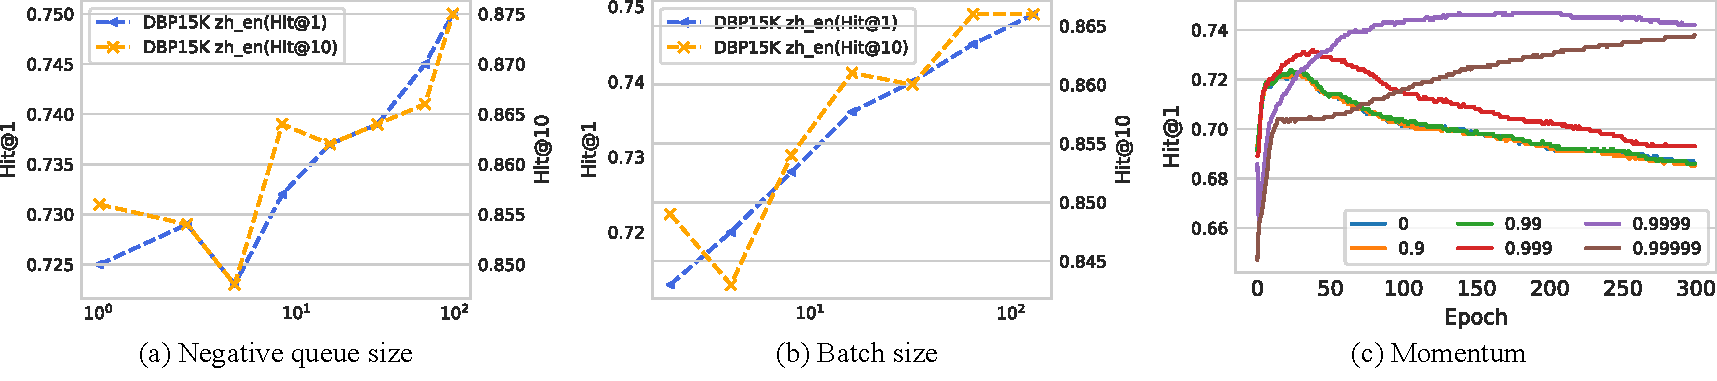
\includegraphics[width=.98\linewidth]{img/selfkg_ablation.pdf}
    \caption{Study on (a) negative queue size, (b) batch size, and (c) momentum on DBP15K$_{\text{zh\_en}}$. (c) presents the test Hit@1 curve throughout the training epochs.}
    \label{fig:size_study}
    %\vspace{-2mm}
\end{figure*}

\begin{figure}
    \centering
        \setlength{\abovecaptionskip}{2mm}
        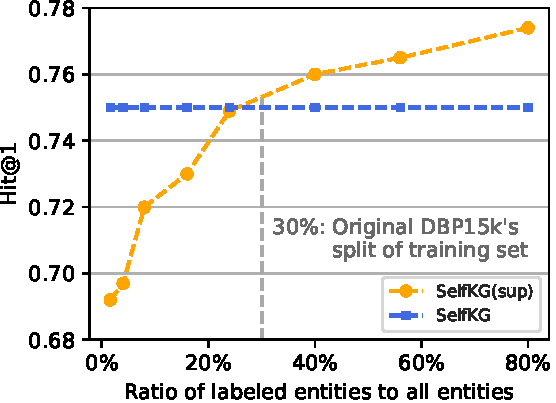
\includegraphics[width=0.9\linewidth]{img/sup.pdf}
        \caption{\solution vs. \solution(sup) on DBP15K. \textmd{\solution works well in a low-data resource setting.}}
        \label{fig:sup}
        \vspace{-0.4cm}
\end{figure}
% \solution is approximately comparable to its supervised counterpart using 90\% of the original training set.

\vpara{Impact of hyper-parameters.} 
The main hyper-parameters in \solution are 1) negative queue size and batch size (which influence the capacity of negative samples), and 2) momentum coefficient $m$ that controls \solution's training stability.

As pointed out in Theorem~\ref{th:asm} and~\ref{th:nasm}, the error term of contrastive loss decays with $\mathcal{O}(M^{-2/3})$, which indicates the importance of enlarging the number of negative samples. Fixing batch size to 64, we change the sizes of the negative queue and derive the curve in Figure~\ref{fig:size_study}. The performance increase is not obvious when queue size is between 10$^0$ and 10$^1$; but as it grows to 10$^2$, the improvement becomes significant. Fixing queue size to 64, along the increase of batch size, the improvement is more stable ranging from 10$^1$ to 10$^2$. 
%Nevertheless, besides the computation of loss, enlarging batch size will also add cost to other computation procedures (while enlarging queue size does not).

For momentum coefficient $m$, we discover that a properly large $m$ such as 0.9999 is usually better for \solution. Besides, a proper $m$ is also critical for better training stability (Cf. Figure~\ref{fig:size_study}). A small momentum leads to faster convergence, but also representation collapse and consequent poorer performance. A too-large momentum (e.g., 0.99999) converges too slow.


% \begin{figure}{r}{}
    \centering
    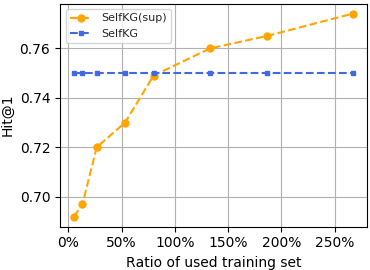
\includegraphics[width=4.5cm]{img/sup.png}
    \caption{Comparison between \solution and \solution(sup). \solution is approximately comparable to its supervised counterpart using 90\% of the original training set.}
    \label{fig:sup}
\end{figure}

\subsection{\solution v.s. Supervised \solution}
In practice, we often encounter low-data resource situations where there is very limited supervision. To justify \solution's scalability, we compare self-supervised \solution with its supervised counterpart \solution(sup) on DBP15K$_{\text{zh\_en}}$ across different data resource settings. \solution(sup) follows the conventional supervised entity alignment methods using Absolute Similarity Metric as presented in Eq.~\ref{eq:asm}.

In our preliminary experiment, we find that the original DBP15k's data split (30\% labels for training and 70\% for testing) is not sufficient to present \solution(sup)'s advantage, resulting in a Hit@1 of 0.744 for \solution(sup) and 0.745 for \solution.
So we construct a new split of DBP15K$_{\text{zh\_en}}$ that contains 20\% for testing and 80\% for constructing different sizes of training set. The result is presented in Figure~\ref{fig:sup}, where the horizontal axis indicates the ratio of training labeled entities for \solution(sup) to all entities. We observe that \solution is approximately comparable to \solution(sup) using an amount of 25\% labeled entities, which accords with our observation in the aforementioned preliminary experiment. When using less than 25\% amount of labeled entities, \solution performs much better than \solution(sup), which demonstrates the effectiveness of \solution in low supervised data resource settings.

%does not surpass \solution as some supervised baselines do, including BERT-INT~\cite{tang2019bert-int}, CEAFF~\cite{CEAFF} and HMAN~\cite{yang2019aligning}. This is because these methods have leveraged side information such as attributes, relations and multi-hop neighbors to boost their performance. In \solution, for simplicity, we only use one-hop neighbors.


% \hhy{ a report of SelfKG runtime and its comparison with baselines, and a more detailed discussion of the approach's limitations}


